Extracting information from free-text written medical texts is a challenging task and has been the subject of numerous publications in recent years \cite{lopez2020covid, wu2020attention, wang2020prediction, slater2021fast, kraljevic2021multi, percha2021modern}. The difficulty of the task stems from the fact that free-text written medical documents follow less the grammatical rules of the written language, contain many abbreviations and spelling mistakes, and the terminology used is typically arising from several languages.

Processing Electric Medical Records written in free requires different Natural Language Processing (NLP) techniques. The information extraction process generally includes two main steps: named-entity recognition (NER) and relation extraction (RE) \cite{sun2018data}. NER aims to identify names or entities (e.g. diseases, medical tests, results of tests), while RE aims to identify relations between them (e.g. symptoms related to diseases).

NER is usually implemented using direct search, rule-based search, machine learning methods or their combinations \cite{grishman1996message}. In practice, searching methods using regular expressions defined by medical experts are most commonly used (e.g. \cite{cohen2019accuracy, fu2020extracting}). The drawback of this approach is that it is difficult to provide a sufficiently general yet specific, complex regular expression that can handle typos and different wordings. Furthermore, they are mainly developed for extracting only one or some predefined keywords. Rule-based methods (e.g. \cite{sahu2018rule, almeida2020rule}) apply rules defined by experts during the search. Although integrating a priori knowledge increases the efficiency of the method, it also significantly limits the application area. Machine learning methods (e.g. \cite{bao2019machine, spasic2020clinical}) also show good performance in recognizing entities; however, their performance is highly influenced by the corpus used for training the model \cite{kormilitzin2021med7}. More recently, for exploring the text descriptions more effectively, text mining, NLP-based (e.g. \cite{carchiolo2019medical, chilman2021text, viani2021natural}), and neural network-based (e.g. \cite{yang2019information, zhu2021utilizing}) methods have been developed, and their use is becoming more widespread. From deep learning methods, mainly the recurrent neural networks (RNN), long short-term memory networks (LSTM), its bidirectional version (Bi-LSTM), the pre-trained transformers models (e.g. Bidirectional Encoder Representations from Transformers, BERT) and convolutional networks (CNN) are used \cite{li2022entity, zhang2022medical}. The authors of these articles generally point out that these models require a considerable computational capacity to build, and the literature review shows that these models perform well mainly in the field of Chinese medical NER due to the specific structure of Chinese written medical text records \cite{chen2022named}. But there are also examples of their use in other languages for named-entity recognition, such as in Spanish or Swedish clinical texts \cite{weegar2019recent}.
 
Considering the application areas, we can find many biomedical application examples, but information extraction from cardiac ultrasound findings is one of the most frequently researched areas. Since the ejection fraction (EF) is one of the most important diagnostic measures and one of the strongest prognostic indicators in patients with cardiovascular disease, several studies aim to extract this diagnostic result (e.g. \cite{garvin2012automated, kim2017extraction, xie2017extracting, vaid2022using}). Garvin et al. \cite{garvin2012automated} used regular expressions for extracting EF values from echocardiogram reports. A similar method is also found in \cite{jonnalagadda2017text}. In \cite{kim2017extraction}, the authors also aimed to extract EF information from three kinds of clinical documents. Based on the characteristics of the corpora, rule-based regular expressions and machine learning-based NLP methods were applied. The authors evaluated the methods from different aspects, including the quantitative evaluations of the extraction of EF mentions, mentions of left ventricular systolic function (LVSF), extraction of EF quantitative values, and EF or LVSF qualitative assessments. Naturally, in addition to the extraction of the EF values, other research was also published that aimed to obtain other cardiac ultrasound characteristics. For example, Wells et al. \cite{wells2014extraction} utilized NLP-based parsing and outlier analysis to extract flow velocities and chamber dimensions. 

In addition to the extraction of predefined characteristics, some studies aimed to extract a broader range of information. In \cite{patterson2017unlocking}, pattern matching was applied to identify the relevant terms, and a concept-mapping algorithm was developed to assign the terms to the appropriate measurement concept. Kaspar et al. \cite{kaspar2019information} investigated how all variables could be extracted from echocardiogram reports and what their quality would be for secondary use. The main conclusion of their study was that data could be extracted from echocardiography documents, but extraction processes should be treated with caution, as the time and effort spent defining every variable may make it dubious.

Based on previous publications, we can see that most of the solutions developed aim at extracting only one or a few predefined results, typically using pattern matching or integrating corpus-specific knowledge. Only two studies \cite{patterson2017unlocking, kaspar2019information} have been published on comprehensive measurement outcome extraction, but they integrate several corpus-specific knowledge.

\vspace{0.5cm}
To overcome these shortcomings, I developed a corpus-independent method to extract quantitative measurement results from echocardiography documents. As the proposed method utilises text-similarity-based mapping, I have analysed different text-similarity measures to find the most suitable measure for information extraction from echocardiography documents. The developed method automatically identifies the name of the measurements and their recorded results in the text, and returns them in a structured way. The efficiency of the method has been evaluated and presented on a large corpus of Hungarian echocardiography documents.

\vspace{0.5cm}
The rest of this chapter is organised as follows: Section \ref{sec:corpus} introduces the corpus used during my research and presents the challenges of extracting information from echocardiography documents. In Section \ref{sec:methods}, different text-similarity measures are evaluated to find the most suitable measure for the develpoed method. Finally, Section \ref{sec:tm_method} discusses the developed method in detail and evaluates it using the corpus introduced in Section \ref{sec:corpus}.

\section{Corpus}
\label{sec:corpus}

Echocardiogram is a sonogram of the heart. It is one of the most widely applied diagnostics test in cardiology: routinely used in diagnosis, management and follow-up of patients with any suspected or known heart disease. Echocardiography reports usually contain two parts in terms as diagnostic content: a semi-structured part where results are usually stored in term-value pairs (e.g.: EN: "Septum: 14 mm", HU: "Szeptum: 14 mm") and a free text part written in natural language (e.g.: EN: Left "ventricular hypertrophy" HU: "Koncentrikus bal kamra hypertrophia"). The form and content of the reports differ in medical institutes. The form and the content of the reports are mainly determined by the habits of the medical assistants and doctors. For example, the test result is separated by a colon from the test name in some sites, while others do not use any separator character. Space characters typically separate different measurement results from each other, but other separator characters, such as semicolons, can also be found. Furthermore, even within one site, the same test result can be recorded with or without a unit of measurement in the reports. There is also a wide variation in how missing data are marked; furthermore, typographical errors increase the variety of the documents. A translated example of an echocardiography document can be seen in Figure \ref{fig:raw_echo_example}.

\begin{figure}[h]
	\centering
        \captionsetup{justification=centering}
	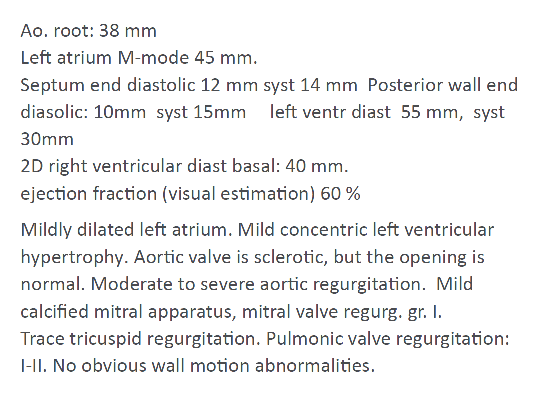
\includegraphics[width=0.75\textwidth]{assets/figures/text_mining/corpus/raw_echo_example.eps}
	\caption{Raw echocardiography report translated to English}
	\label{fig:raw_echo_example}
\end{figure}

The effectiveness of my proposed method was evaluated by processing 20,074 echocardiography reports. The document set was collected in a Hungarian hospital and contained all findings recorded between 2017 and 2021. The findings were anonymised, and did not contain any information about the patient or the examining physician. As there is no publicly available benchmark dataset to evaluate such methods, a dataset had to have been collected, and, as all proposed methodologies does not contain any language-dependent processing activity and the proposed method can be used for documents written in any language, the collected dataset was adequate for evaluation.

\subsection{Challenges of processing echocardiography documents}
\label{sec:challenges}

The methods presented in the introduction of Chapter \ref{chap:text_mining} are widely applicable to extract information from medical documents mainly written in English, however the nature of Hungarian language requires specific tools to extract information from medical documents written in Hungarian. In this section, I discuss the How To-s and challenges of the general extraction process of echocardiography reports, and also present some Hungarian language specific problems.

% Generally, the main task of information extraction from medical texts is to identify particular types of names, terminologies or symbols (term extraction, named-entity recognition, NER) and the relation between them (relation extraction, RE). Successful term identification is essential and has been recognized as a bottleneck in text mining. The process of term identification is usually achieved in three steps: the first step is term recognition where possible term candidates are identified; the second step is term classification where the candidates are classified based on pre-defined rules; and the last step is term mapping where the candidates are checked whether they are valid terms or not.

\vspace{1.0cm}

As I mentioned before, the semi-structured part of echocardiography reports contains medical information in term–value pairs separated by colon. The term part refers to the identifiable named entities and the value part refers to the measured and recorded value for that named entity. The measured value may also contain a unit of measurement. However, based on the extraction approach, various challenges emerge aside from typographical errors during term extraction. These challenges are described in detail in the following subsections.

\subsubsection*{Articles}

A common characteristic of the English and the Hungarian language is the use of "a” article before adjectives and nouns (in Hungarian "a”/”az” pair is used and in English "a”/”an” pair is used). In most case the use of the "a” article does not pose a problem, however, in case of echocardiogram reports, "A" (A wave) is the peak velocity flow in late diastole caused by atrial contraction. Furthermore, in Hungarian language "e” expletive is also present, but in echocardiography reports "E" (E wave) stands for the peak velocity blood flow from gravity in early diastole.

\subsubsection*{Typographical errors}

The lack of a unified recording interface infers many typographical errors which need to be taken into account during term extraction. Most frequent typographical errors can be resolved by using a dictionary which contains the original form of medical terms and their synonyms. If the similarity of the written expression to any term of the dictionary is within an acceptable margin, it is resolvable.

\subsubsection*{Missing whitespaces}

As a form of typographical error, missing whitespaces can also occur between terms, values and units (e.g. EN: "Left ventricular end-diastolic diameter43.: mm", HU: "Bal kamra diast.átm43.: mm"). If the text processing method is word-based, missing whitespaces have a huge impact on the success of processing. This problem can be handled by inserting separator space characters into the text during text cleaning, if text cleaning is applied.

\subsubsection*{Recognition of composite terms}

Not only typographical errors make it harder to extract information from echocardiography reports. Based on the assumption, that named-entities follow the term-value pair structure, it is possible to extract the greater part of named entities. However, special cases are also present in echocardiography reports mostly because of the habits of the recording individual. Such a composite term can be described in \textit{prefix–term1–term2-value1–value2–common\_unit} form (e.g. EN: "left ventricular end-diast/end-syst diameter: 54/35 mm", HU: "bal kamra diast/syst átmérő: 54/35 mm") where the recording individual aggregates two somewhat related terms. In this case the identified term should be interpreted as \textit{prefix–term1–value1–unit} and \textit{prefix–term2–value2–unit}.

Other composite terms can also be present. For example EN: "ejection fraction Teichholz: \SI{56}{\percent}, Simpson \SI{52}{\percent"}, HU: "ejekciós frakció Teichholz: \SI{56}{\percent}, Simpson: \SI{52}{\percent"} can be described as \textit{prefix–term1–value1–unit–term2–value2–unit} or "E/A: 0.4/0.8 m/s" can be describe as \textit{term1–term2–value1–value2–unit}.

Furthermore, expletives are also commonly used (e.g. EN: "left atrium: 42 mm (apical 4Ch: 43x75mm)", HU: "Bal pitvar: 42 mm (csúcsi nézetből: 43x57 mm)") which makes composite term recognition even harder. A possible approach to process composite terms is to define some basic rules and process echocardiography documents based on these rules.

% during the term mapping process. The identified and classified term candidates must be checked whether they are valid terms or not using the aforementioned dictionary of terms. This dictionary is usually created with the help of a medical expert and contains more terms from the field of interest.

%in our case the field of cardiology, probably present in some form in echocardiography reports and defines synonyms for the terms.

% The extracted terms can be compared against the values of the dictionary. The distance for two strings can be calculated by any of the measures introduced in Section \ref{sec:metrics}, If the measured distance is lower than a specified distance threshold, the term is considered valid and identified. This threshold parameter can be the lowest, non-zero intra-distance of the terms stored in the dictionary.

\section{Evaluation of different text similarity metrics}
\label{sec:metrics}

To develop a text-similarity-based information extraction method, exact matching is not a viable option, as it is not capable of finding synonyms, typos, and abbreviations of the search term. For this purpose, I examined and compared different text similarity metrics applied in the field of NLP. My goal was to determine which similarity metrics present the highest gain in terms of searching for echocardigoraphy documents containing a given keyword or its misspelled, abbreviated or synonym form. 

\subsection{Included metrics}

The basic distance metrics included in my case study are widely used metrics in the field of NLP. The metrics of the study were the following: Longest Common Subsequence (LCS), Levenshtein distance (LD), weighted Levenshtein distance (WLD), Jaro-Winkler distance, and cosine distance. In the following, these metrics and the principles behind them are introduced in detail.

\subsubsection*{Longest Common Subsequence}

Longest Common Subsequence (LCS) is one of the simple metrics measuring the similarity of two strings. It finds the longest subsequence of characters present in both texts. To measure the similarity of the two strings, the actual common subsequence is irrelevant, only the length of it is taken into account \cite{lonardi2010string}. For example, both "cardi" and "ardil" are subsequences of "cardiology" and their length in both cases equals to five. The term subsequence is defined as follows. Given a sequence $a=a_1,  \dots, a_k$. Another $b=b_1, \dots,b_m$ sequence is a subsequence of $a$ if such a strictly increasing sequence of indices ($i_1,\dots,i_m$) of $a$ exists that for all $j=1,\dots,m$, $a_{i_j}=b_j$. This metric also takes the cases into account where some characters are omitted, but it cannot recognise swapped characters.

\subsubsection*{Levenshtein distance}

The Levenshtein distance \cite{miller2009levenshtein, piskorski2007string} is a more complex dissimilarity metric that counts the number of the edits that are needed to transform an $s_1$ string into another $s_2$ string. The Levenshtein distance takes the following operations into account: insertion, deletion, and substitution of characters. The Levenshtein distance works basically on single words, however, it is not restricted to those: it can also be calculated for strings of any type.

$lev_{s_1,s_2}(|s_1|,|s_2|)$ denotes the Levenshtein distance of strings $s_1$ and $s_2$, where $|s_1|$ and $|s_2|$ yield the lengths of strings $s_1$ and $s_2$, and $lev_{s_1,s_2}(i,j)$ for each $i,j \in \mathbb{N}$ is calculated as:

\begin{equation}
	lev_{s_1,s_2}=
	\begin{cases}
		max(i,j) & \text{if } min(i,j)=0 \\
		min \begin{cases}
		lev_{s_1,s_2}(i-1,j)+1  \\
		lev_{s_1,s_2}(i,j-1)+1  \\
		lev_{s_1,s_2}(i-1,j-1)+1_{(s_{1i} \neq s_{2j})} 
	\end{cases} & \text{otherwise}
	\end{cases}
	\label{eq:levenshtein}
\end{equation}

The inclusion of the Levenshtein distance was motivated by the fact that in medical texts the Latin medical terms are probably written, to some degree, in a way similar to spoken-language, and this kind of difference between two words can be easily caught by the use of the Levenshtein distance.

\subsubsection*{Weighted Levenshtein distance}

The original Levenshtein distance is not flexible enough to consider the magnitude of errors: all edit operations uniformly cost 1. However, practically, not all edits can be considered equivalent. For example, in case of typo correction substituting "r" for "t" should have a smaller cost, since they are located close to each other on a keyboard with QWERTY layout. The weighted Levenshtein distance considers all these aspects as well and sets different costs to the pairs of characters according to the probability of their interchange.

\subsubsection*{Jaro-Winkler distance}

The Jaro-Winkler distance \cite{piskorski2007string} accounts for the lengths of two strings and partially accounts for the type of typographical errors humans make when typing texts. It is calculated in the following way:

\begin{equation}
	d_w(s_1,s_2)=1-sim_w(s_1,s_2)
	\label{eq:winkler_d}
\end{equation}

\begin{equation}
	sim_w(s_1,s_2)=sim_j(s_1,s_2)+lp(1-sim_j(s_1,s_2))
	\label{eq:winkler_sim}
\end{equation}
where $sim_j$ is the Jaro similarity for $s_1$ and $s_2$ strings, $l$ is the length of a maximum 4 characters long common prefix and $p$ is a constant scaling factor with a standard value of $0.1$. The Jaro similarity ($sim_j$) is calculated as:

\begin{equation}
	sim_j(s_1,s_2)=
	\begin{cases}
		0                                                                            & \text{if } m=0   \\
		\frac{1}{3} \left( \frac{m}{|s_1|} + \frac{m}{|s_2|} + \frac{m-t}{m} \right) & \text{otherwise} 
	\end{cases}
	\label{eq:jaro_sim}
\end{equation}
where $|s_i|$ is the length of $s_i$, $m$ is the number of matching characters and $t$ is half of the number of transpositions. The concept of matching and transpositions is detailed in \cite{piskorski2007string}.

The Jaro-Winkler distance metric results in smaller distance values for those two strings that match from the beginning in length l. I decided to analyse the applicability of this kind of distance metric as well, because my hypothesis based on the manual review of a pre-selected sample document was that typing errors are more common toward the end of the words.

\subsubsection*{Cosine similarity}

The cosine similarity is also a widely used similarity metric for comparing two strings. For example, it was used in anomaly detection in web documents \cite{friedman2007anomaly}, in content-based recommender systems \cite{zenebe2009representation}, and even it was used for pattern recognition in medical diagnoses \cite{ye2011cosine}. In the case of calculating cosine similarity, the strings are represented as vectors, and the similarity is calculated from the angle enclosed by the vectors. More formally, the cosine similarity is defined as the inner product of two vectors divided by the product of their lengths. To get the cosine similarity of two strings, the compared strings first have to be projected to an high-dimensional (typically several hundred dimensions) vector space. I achieved it by applying word embedding.

Word embedding \cite{mikolov2013distributed} is one of the most popular representations of document vocabulary as it is capable of capturing the context of a word in a document, semantic and syntactic similarities or even relations between words. It provides an efficient representation in which similar words have similar encodings. As a result, the words that occur in a similar context will be represented as similar high-dimensional vectors and they tend to have high cosine similarity, as well.

I used the FastText word embedding library developed by Facebook AI Research (FAIR) team to calculate the high-dimensional vector representations for words occurring in medical texts. FastText is an extension of the Word2Vec model proposed by Google \cite{mikolov2013distributed}. It uses a two-layer neural network for high-dimensional representation. The input of FastText is the word to be mapped with the surrounding text and the output is a high-dimensional representation of the word. The key difference between Word2Vec and FastText is the use of n-grams: Word2Vec only learns from complete words found in the training corpus, while FastText not only considers the complete words, but also the n-grams that are found within each word.

Having the high-dimensional representations of the strings to be compared, the cosine similarity can be calculated by Eq. \ref{eq:cosine}.

\begin{equation}
	sim(\textbf{S}_1,\textbf{S}_2)=\frac{\sum_{i=1}^{n}s_{1i} s_{2i}}{\sqrt{\sum_{i=1}^{n}s_{1i}^2}\sqrt{\sum_{i=1}^{n}s_{2i}^2}}
	\label{eq:cosine}
\end{equation}
where vectors $\textbf{S}_1=[s_{11},s_{12},\dots,s_{1n}]$ and $\textbf{S}_2=[s_{21},s_{22},\dots,s_{2n}]$ are the high-dimensional vector representations of strings (in my case, words) $s_1$ and $s_2$. 

The examination of cosine similarity was based on the fact that although the same condition may be formulated differently in medical descriptions, but the text surrounding the condition is most likely similar. My hypothesis was that the different descriptions of the same medical terms (e.g. Latin and Hungarian forms of the same term) will get high cosine similarity value. As the similarity of the synonyms cannot be expressed by the application of the similarity metrics presented before, I had great hopes for cosine similarity.

\subsection{Evaluation process}
\label{sec:eval_tm}

I had to select the most appropriate text similarity metric as my main goal was to develop a text-similarity-based information extraction method. This choice was made by processing the results of the evaluation process presented by Figure \ref{fig:evaluation_workflow}. The evaluation was done on the corpus presented in Section \ref{sec:corpus}. The number of unique expressions found in the original 20,074 reports was 25,380. 

\begin{figure}[h]
	\centering
        \captionsetup{justification=centering}
	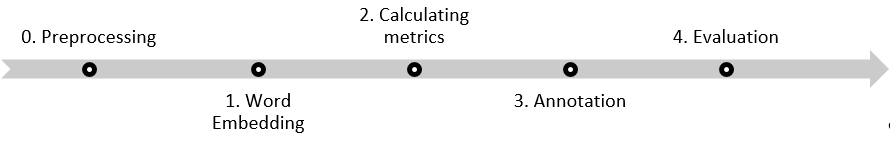
\includegraphics[width=\textwidth]{assets/figures/text_mining/measures/workflow.png}
	\caption{Workflow of the evaluation}
	\label{fig:evaluation_workflow}
\end{figure}

All echocardiography reports have been preprocessed as the zeroth step. The aim of \textit{Preprocessing} was to identify the measurements recorded as numerical values and to connect them to their units. The different measured values were replaced with a unified special character to not differ in the preprocessed text. They can be mapped back to their original values at a later step. This way, the variability of the text resulting from different measurement results was significantly reduced, and the size of the vocabulary was also reduced to 15,105 expressions.

The next step was the design and the execution of \textit{Word Embedding}. The applied FastText-based neural network was tested with different parameter settings. The best performing neural net utilised a skipgram model with negative sampling. The number of negative samples was 5 and the sampling threshold applied was $10^{-4}$. The learning rate was set to $0.05$ with a rate of $100$ for updating the learning rate. With 20 epochs and a window size of 5, all the words of the preprocessed documents have been mapped to 100-dimensional vectors.

To evaluate the usefulness of the similarity metrics presented in Section \ref{sec:metrics}, 10 medical terms considered as important search keywords have been selected by the collaborating doctors personal preferences. These terms were the following: regurg (insuff), hypokinesia (hypokinézis), akinesia (akinézis), shunt (shunt), bicuspidal (bicuspidalis), thrombus (thrombus), stenosis (szűkület), systolic (systoles), mitral (mitrális), and wallmotion abnormality (falmozgászavar). It is important to note that all these medical term were given according to the Hungarian terminology, where all of them are expressed with one word. Furthermore, it may seem that the set of selected words is rather small, but in a later step, doctors have to manually annotate the resulting similar words.

In the second step, \textit{Calculating metrics}, the 1,000 nearest matches have been determined for every investigated distance metric and for all of the terms presented in the previous paragraph. All calculated distance values have been converted to similarity values, and the converted values have been normalised to the range of $[0,1]$. A similarity threshold of $0.65$ has also been introduced to limit the number of candidate words.

%have been calculated for the 1,000 nearest matches of the previously presented keywords. 

%For the final evaluation, all calculated distance values have been converted to similarity values and the converted values have been normalised to the range of $[0,1]$.

The third step was \textit{Annotation}. With the help of a cardiologist, a subset of the closest words has been annotated according to the following annotation rules:
\begin{itemize}
	\item \textit{2}, if the found word was considered identical to the term searched for (e.g. alternative forms, abbreviations, typos)
	\item \textit{1}, if based on the found word, the cardiologist would consider checking the report containing it to decide whether the report contains relevant information or not, and finally
	\item \textit{0}, if the found word was considered irrelevant.
\end{itemize}
The difficulty of the task is shown by the fact that the evaluation of the similar words found for these 10 search words required annotation for 8,647 similar words.

The final step was the \textit{Evaluation}, where the ROC (Receiver Operating Characteristic) curves have been plotted and the corresponding AUC (Area Under the Curve) values have been calculated based on the annotation labels for each search word: two values for each. The first called \textit{hard evaluation} was calculated where only the words labelled \textit{2} were considered matches, and the second one was the \textit{soft evaluation}, where the words labelled as \textit{1} and \textit{2} were also considered relevant matches.

\subsection{Results of the evaluation}

The results of the \textit{Evaluation} step can be seen in this section.

Table \ref{tab:number_of_candidates} shows the resulted number of candidate words in case of setting the similarity threshold equal to $0.65$. $N_C$ yields the number of candidates, $N_H$ and $N_S$ the number of the true positive terms for the hard and soft evaluations respectively. The corresponding AUC values for the results presented in Table \ref{tab:number_of_candidates} can be seen in Table \ref{tab:auc_values}. The notation "-" means that with this parameter setting, exclusively real positive candidates were selected and therefore the area under the ROC curve could not be calculated. As we can see, the LCS, Levenshtein, and weighted Levenshtein distances are more capable of distinguishing the true positive candidates from the false positive ones. The advantage of using the weighted version of the Levenshtein distance versus the basic one cannot be observed.

\begin{table}[h!]
	\centering
	\caption{The number of candidate words in case of applying different similarity metrics and evaluation methods, while setting the similarity threshold equal to $0.6$5. %$N_C$ yields the number of candidates, $N_H$ and $N_S$ the number of the true positive terms for the hard and soft evaluations respectively.
 }
	\label{tab:number_of_candidates}
	\resizebox{\textwidth}{!}{
		\begin{tabular}{l|rrrrrrrrrrrrrrr} \toprule
			& \multicolumn{15}{c}{Number of candidate words} \\
			& \multicolumn{3}{c}{LCS} & \multicolumn{3}{c}{Levenshtein} & \multicolumn{3}{c}{weighted Lev.} & \multicolumn{3}{c}{Jaro-Winkler} & \multicolumn{3}{c}{Cosine} \\
			Term                   & \multicolumn{1}{c}{$N_C$} & \multicolumn{1}{c}{$N_H$} & \multicolumn{1}{c}{$N_S$} & \multicolumn{1}{c}{$N_C$} & \multicolumn{1}{c}{$N_H$} & \multicolumn{1}{c}{$N_S$} & \multicolumn{1}{c}{$N_C$} & \multicolumn{1}{c}{$N_H$} & \multicolumn{1}{c}{$N_S$} & \multicolumn{1}{c}{$N_C$} & \multicolumn{1}{c}{$N_H$} & \multicolumn{1}{c}{$N_S$} & \multicolumn{1}{c}{$N_C$} & \multicolumn{1}{c}{$N_H$} & \multicolumn{1}{c}{$N_S$} \\ \midrule
			regurg                 & 17                        & 15                        & 15                        & 15                        & 15                        & 15                        & 15                        & 15                        & 15                        & 103                       & 25                        & 29                        & 155                       & 54                        & 91                        \\
			hypokinesia            & 76                        & 69                        & 73                        & 58                        & 53                        & 55                        & 34                        & 33                        & 34                        & 470                       & 297                       & 316                       & 489                       & 268                       & 276                       \\
			shunt                  & 6                         & 6                         & 6                         & 6                         & 6                         & 6                         & 11                        & 6                         & 6                         & 167                       & 19                        & 20                        & 466                       & 48                        & 54                        \\ 
			bicuspidal             & 6                         & 2                         & 2                         & 6                         & 2                         & 2                         & 5                         & 2                         & 2                         & 135                       & 3                         & 4                         & 1000                      & 3                         & 3                         \\  
			thrombus               & 25                        & 25                        & 25                        & 22                        & 22                        & 22                        & 23                        & 23                        & 23                        & 191                       & 41                        & 49                        & 97                        & 42                        & 52                        \\    
			stenosis               & 7                         & 6                         & 6                         & 6                         & 6                         & 6                         & 6                         & 6                         & 6                         & 237                       & 15                        & 19                        & 1000                      & 15                        & 52                        \\    
			systolic               & 50                        & 19                        & 39                        & 45                        & 19                        & 34                        & 39                        & 17                        & 27                        & 259                       & 27                        & 83                        & 136                       & 30                        & 89                        \\     
			akinesia               & 5                         & 4                         & 4                         & 5                         & 4                         & 4                         & 2                         & 1                         & 1                         & 306                       & 35                        & 36                        & 549                       & 40                        & 62                        \\     
			mitral                 & 27                        & 15                        & 15                        & 22                        & 13                        & 13                        & 12                        & 10                        & 10                        & 519                       & 20                        & 25                        & 151                       & 20                        & 23                        \\     
			wallmotion abnormality & 33                        & 28                        & 33                        & 23                        & 18                        & 23                        & 19                        & 17                        & 19                        & 269                       & 28                        & 68                        & 220                       & 28                        & 8                         \\ \bottomrule
		\end{tabular}}
\end{table}

\begin{table}[h!]
	\centering
	\caption{AUC values in case of applying different similarity metrics and evaluation methods, while setting the similarity threshold equal to $0.65$.}
	\label{tab:auc_values}
	\resizebox{\textwidth}{!}{
		\begin{tabular}{l|cccccccccc} \toprule
			\multicolumn{1}{c}{} & \multicolumn{10}{c}{AUC}                                                                                            \\
			& \multicolumn{2}{c}{LCS} & \multicolumn{2}{c}{Levenshtein} & \multicolumn{2}{c}{weighted Lev.} & \multicolumn{2}{c}{Jaro-Winkler} & \multicolumn{2}{c}{Cosine} \\
			Term                   & Hard   & Soft   & Hard   & Soft   & Hard   & Soft   & Hard   & Soft   & Hard   & Soft   \\ \midrule
			regurg                 & 1.0000 & 1.0000 & -      & -      & -      & -      & 0.9954 & 0.9646 & 0.8894 & 0.8398 \\
			hypokinesia            & 0.6004 & 0.7032 & 0.6038 & 0.8545 & 0.1818 & -      & 0.8483 & 0.8609 & 0.8657 & 0.8695 \\
			shunt                  & -      & -      & -      & -      & 0.9333 & 0.9333 & 0.9968 & 1.0000 & 0.9041 & 0.9143 \\
			bicuspidal             & 1.0000 & 1.0000 & 0.8750 & 0.8750 & 1.0000 & 1.0000 & 0.9975 & 0.9790 & 0.9997 & 0.9997 \\
			thrombus               & -      & -      & -      & -      & -      & -      & 0.9865 & 0.9789 & 0.9519 & 0.8850 \\
			stenosis               & 0.6667 & 0.6667 & -      & -      & -      & -      & 0.9688 & 0.9138 & 0.7919 & 0.7464 \\
			systolic               & 0.9440 & 0.7389 & 0.9413 & 0.8396 & 0.7701 & 0.7191 & 0.9120 & 0.9371 & 0.8041 & 0.5675 \\
			akinesia               & 1.0000 & 1.0000 & 1.0000 & 1.0000 & 1.0000 & 1.0000 & 0.8741 & 0.8507 & 0.7622 & 0.6622 \\
			mitral                 & 0.9778 & 0.9778 & 0.9829 & 0.9829 & 0.8000 & 0.8000 & 0.9704 & 0.9670 & 0.8729 & 0.8441 \\
			wallmotion abnormality & 0.9286 & -      & 0.7000 & -      & 0.9118 & -      & 0.8718 & 0.9606 & 0.9269 & 0.9243 \\
			\bottomrule
		\end{tabular}
	}
\end{table}

Comparing the two similarity metrics that selected more words as candidates, namely the Jaro-Winkler distance and the cosine distance, we can see that the application of the Jaro-Winkler distance is more appropriate in this topic. After manually reviewing the results, I have established, that although the cosine distance can extract completely different word synonyms as well, they appear in the result set with lower similarity values. Consequently, the false positive results appear with greater similarity values in the results set than the completely different forms of synonyms. Based on my findings, I had to reject the former hypothesis that cosine similarity based on the applied FastText embedding can significantly improve keyword-based search in medical texts. The results can be explained by the fact that the contexts surrounding synonyms are probably different for those medical texts that use different expressions for the same content.

\begin{figure}[h]
	\centering
        \captionsetup{justification=centering}
	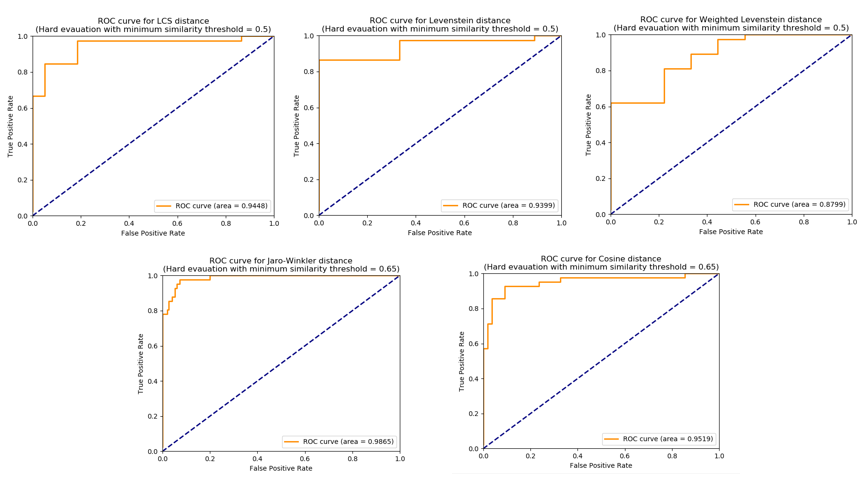
\includegraphics[width=\textwidth]{assets/figures/text_mining/extraction/roc_results.png}
	\caption{ROC analysis of finding the term "thrombus" using different similarity measures.}
	\label{fig:roc_values}
\end{figure}

The results presented in Table \ref{tab:number_of_candidates} and Table \ref{tab:auc_values} show that for the LCS, Levenshtein and weighted Levenshtein metrics a lower, and for Jaro-Winkler and cosine similarity metrics a higher threshold value has to be applied to get enough true positive candidate words in a way to get good enough AUC value for the classifier. For example, in Figure \ref{fig:roc_values}, the ROC curves for searching for the word "thrombus" is presented. For finding more positive samples the similarity threshold for LCS, Levenshtein, and weighted Levenshtein distances was decreased to $0.5$, while the threshold for Jaro-Winkler and cosine similarities was left equal to $0.65$. The number of the true positive candidates in this case were: $N_{LCS}=39$, $N_{Levenshtein}=37$, $N_{wLevenshtein}=37$, $N_{Jaro-Winkler}=41$, $N_{Cosine}=42$. Comparing the results to data listed in Table \ref{tab:number_of_candidates} and Table \ref{tab:auc_values}, we can see, that as the threshold decreased for the first three similarity metrics, the number of positive candidates increased, however the area under the ROC curve decreased.

My results showed that the Jaro-Winkler and cosine distances, at the same similarity threshold, can discover more candidate words to be similar to the keyword. Although a classifier based on the Common Subsequence, Levenshtein or weighted Levenshtein distances with higher similarity thresholds is more capable of distinguishing the true positive candidates from the false positive ones, with these high thresholds, these metrics provide less true positive results. Furthermore, my results pointed out, that the weighted Levenshtein distance cannot substantially contribute to improving the result of the Levenshtein distance.

Considering the applicability of the cosine distance based on the FastText word embedding, I found that the exploration of synonyms requires a significantly lower threshold, which results in the decrease of the efficiency of the classifier, as well.

The most promising distance metric was the Jaro-Winkler distance, which can return a relatively large number of documents in a way that the distinctive ability of the classifier still remains high. There, the developem text mining-based information extraction method utilises the Jaro-Winkler distance.

\section{The proposed text mining-based information extraction method}
\label{sec:tm_method}

Going beyond the limitations of methods introduced at the beginning of Chapter \ref{chap:text_mining}, I developed a generally applicable text mining method for extracting numerical test results with their descriptions from free-text-written echocardiography reports. The proposed method breaks with regex-based information extraction methods and employs corpus-independent text mining techniques to extract information from medical texts. It automatically detects expressions containing textual descriptions of the test results and pairs them with their numerical measurement results. The identification of candidate terms is performed by using similarity-based matching to match them to standardised clinical terms. The similarity-based mapping uses Jaro-Winkler distance and makes it possible to handle typos, synonyms and abbreviations flexibly; therefore, the efficiency of the information extraction is significantly increased. Additionally, the proposed method can extract multiple information from the documents by a single search, and a repetitive scan is not needed. The proposed method is mainly recommended for the rapid processing of large volumes of echocardiography findings, such as to support medical research or to verify patient selection criteria for clinical trials quickly.

The applicability of the proposed method was tested by processing the corpus presented on Section \ref{sec:corpus}. Figure \ref{fig:extraction_example} shows how the proposed method extracts and transforms the measurement results of the raw echocardiography document into a uniform and structured form. 

\begin{figure}[h]
	\centering
        \captionsetup{justification=centering}
	\begin{subfigure}[b]{0.60\textwidth}
		\centering
		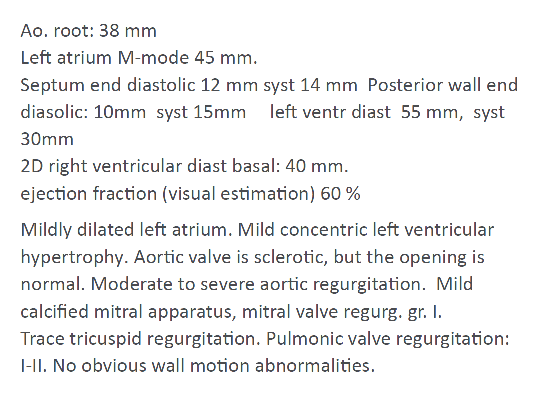
\includegraphics[width=\textwidth]{assets/figures/text_mining/corpus/raw_echo_example.eps}
		\caption{Echocardiography report}
		\label{fig:extraction_example_a}
	\end{subfigure}
	\hfill
	\begin{subfigure}[b]{0.36\textwidth}
		\centering
		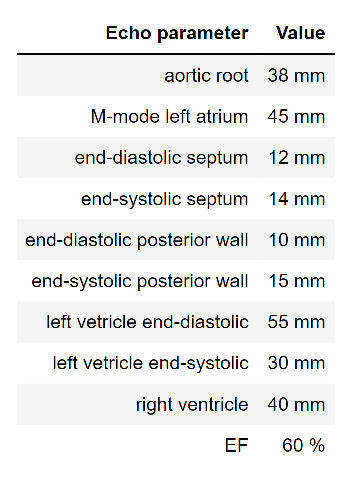
\includegraphics[width=\textwidth]{assets/figures/text_mining/corpus/extracted_echo_example.eps}
		\caption{Extracted result}
		\label{fig:extraction_example_b}
	\end{subfigure}
	\caption{The raw echocardiography report (a) and the extracted measurement results (b).}
	\label{fig:extraction_example}
\end{figure}

\subsection{Extracting measurement results from echocardiography documents}
\label{subsec:extracting}

% My aim was to develop a generally applicable text mining-based information extraction method to extract term-value pairs from echocardiography documents.

The steps of the proposed method can be seen on Figure \ref{fig:extraction_workflow}. The steps are the following: (1) corpus-independent preprocessing of echocardiography documents; (2) identification of the candidate technical terms; (3) refinement of the identified candidate terms; (4) mapping the candidate terms for the standardised clinical terms; (5) validation of the extracted terms and their measured results. The steps are detailed in the next paragraphs.

\begin{figure}[h]
	\centering
        \captionsetup{justification=centering}
	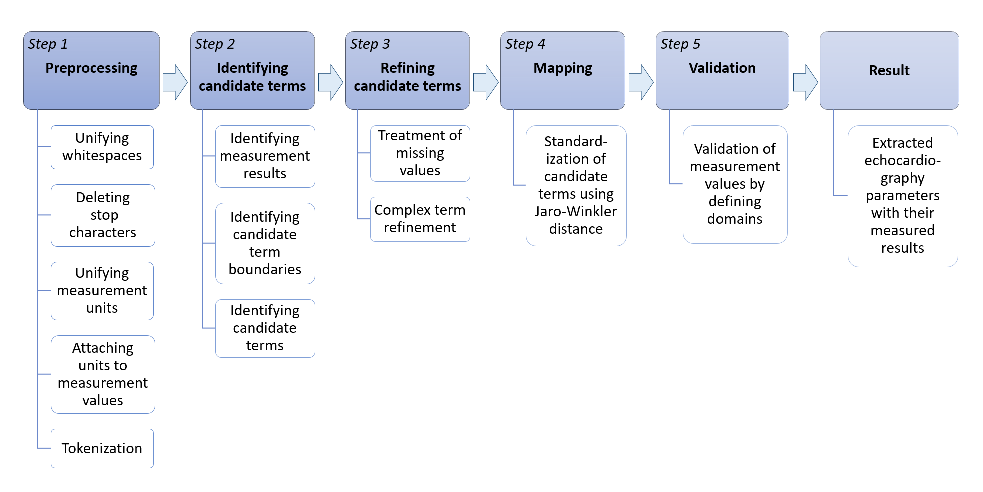
\includegraphics[width=\textwidth]{assets/figures/text_mining/extraction/workflow.eps}
	\caption{The steps of the proposed text mining method.}
	\label{fig:extraction_workflow} 
\end{figure}

\textbf{Preprocessing:} The preprocessing phase includes such text cleaning activities which aim at unifying the text and minimising the differences between them arising from the recording habits. Therefore, in the first step, the whitespaces are unified and the unneeded characters are deleted according to a predefined character list (\textit{stop characters}). The list of stop characters contains all characters that do not contain any information for the measured results. The list I used and recommend contains the following items: colon, brackets, quotation marks, TAB character and ENTER character. As it can be seen, the dot and comma characters are not the elements of the list because they may also denote decimal separator characters. However, it is important to emphasise that the colon character is the element of the list, and it is deleted at this stage, as the algorithm does not rely on the fact that the measurement results are separated from the name of the measurement by a colon or not. 

The next step is to standardise the units of measurement based on a list predefined by an expert. As part of the standardisation, units of measurement containing numbers will be replaced to not contain numbers. (e.g. "mm2" is replaced by "sqrmm"). After standardising the units of the measurements, they are glued to the preceding numerical values (e.g. "85 cm/sec" is replaced by "85cm/sec"). In this way, we can assume that words beginning with a numerical value contain measurement results (typically with their unit of measurement). These "words" are considered \textit{possible measurement results} and are called PMR tokens.

Following this, the cleaned documents are split into tokens, which are text fragments separated by whitespace characters. This tokenised and preprocessed text serves as the basis for the named entity recognition at the next phase.

\textbf{Identifying candidate terms:} This step aims to identify those text fragments that may indicate the names of ultrasound parameters. The proposed method assumes that the description of the measurement precedes the recording of the measurement result. Texts with lengths up to $n$ tokens located between PMR tokens or preceding the first PMR token are considered text fragments that may record the name of a parameter. They are called \textit{echocardiography parameter candidates} (EPCs). The possible maximal number of the words ($n$) in EPCs is an input parameter of the method and can be established based on the corpus. After the identification, the EPCs and the PMRs are stored in structured form for subsequent processing. We have to note that EPCs do not correspond to the exact names of measurements in all cases; they may still contain complex terms, typos, and abbreviations. 

\textbf{Refining candidate terms:} In this phase, complex EPCs will be refined using text fragmentation methods. 

If an EPC contains a token describing a unit of measure, it must be divided into two or more parts, since in this case, we can assume that the first part of the term candidate refers to an empty measurement result, while the second part contains another measurement. Given the "A cm/sec EF \SI{62}{\percent}" example, the complex EPC contains the "A cm/sec EF" string, which will be cut into two EPCs, which are "A cm/sec" and "EF". The original PMR value ("\SI{62}{\percent}") will be connected to the EPC "EF", and the first part of the text will be stored as "A" and "cm/sec" EPC-PMR pair. If the first part contains more than one unit of measurement, then the splitting has to be done recursively in several steps.

The next activity is to recognise and handle the \textit{complex term–measurement sequences}. The forms of the complex sequences may be as follows:

\begin{itemize}
	\item \textit{term1–term2–result1–result2} sequence: e.g. "left ventricular diameter end-diastolic/end-systolic 54/35mm",
	\item \textit{term1–result1–subterm2–result2} sequence: e.g. "ejection fraction Teichholz \SI{56}{\percent} Simpson \SI{52}{\percent}".
\end{itemize}

The occurrences of complex sequences are searched using predefined rules. If the sequence fits any of the rules, then the complex sequence is converted into simple term-result pairs, and the refined EPCs with their PMRs are stored.

\textbf{Mapping:} As identified EPCs may contain typos and abbreviations, the next phase of the text processing aims to clarify and standardise them. For achieving this goal, EPCs are mapped onto a dictionary containing the standardised names of the ultrasound parameters and their synonyms (e.g. "end-diastolic posterior wall", "LVPWd"). The dictionary can be based on any standardised collection of clinical terms (e.g. SNOMED CT \cite{donnelly2006snomed}), or it can also be defined by experts.

In Section \ref{sec:metrics} I showed that among the different distance metrics, the Jaro-Winkler distance achieves the best results in named entity recognition performed in echocardiography documents. Therefore, in the present method, Jaro-Winkler distance-based mapping is used.

For each EPC, a distance matrix is calculated, which contains the Jaro-Winkler distances between the EPC string and the elements of the standardised dictionary. If the smallest value of the distance matrix is less than a predefined threshold value ($\alpha$), then the EPC is mapped to the standardised name of the most similar dictionary element. Otherwise, the EPC is discarded.

\textbf{Validation:} During this step, the PMR values are validated by defining a range of interpretations for each ultrasound parameter. If the measured value does not fall within its domain, it will be treated as a possible error.

As a result of the previous steps, the measurement results extracted from the echocardiography documents are available in a structured format (measurement name - measurement result pairs). This structured format allows users (e.g. physicians) to process and use the results in their future work easily (e.g. patient selection for studies or time-series comparison of results). 

\subsection{Evaluation of the proposed text mining-based information extraction method}
\label{sec:eval_text_mining}

The effectiveness of the proposed method was evaluated by processing the corpus presented in Section \ref{sec:corpus}. During the evaluation, the effectiveness of the extraction of 12 commonly measured echocardiography parameters was examined. These parameters were: aortic root diameter (aorta gyök), M-mode left atrial diameter (Bal pitvar), end-diastolic septum thickness (Septum végdiast), end-systolic septum thickness (Septum syst), left ventricle end-diastolic diameter (Bal kamra diast. átmérő), left ventricle end-systolic diameter (Bal kamra syst. átmérő), end-diastolic posterior wall thickness (Hátsófal végdiast.), end-systolic posterior wall thickness (Hátsófal syst.), right ventricle end-diastolic diameter (Jobb kamra), A-wave (A), E-wave (E), and left ventricular ejection fraction (EF). 

The threshold for the maximal number of the tokens in EPCs was set to $n=4$, and the threshold parameter for the Jaro-Winkler distance between the EPCs and the standardised terms was set to $\alpha=0.1$. The first parameter was determined as the suggestion of the medical expert, while the second one was obtained as an empirical fact from my previous study \cite{vathy2020efficiency}. The cardiac ultrasound documents were processed in a single iteration, and the detected EPCs were mapped into a standardised dictionary. The dictionary used for mapping contained 56 synonyms for the 12 terms. 

After performing the proposed method, the evaluation was carried out as follows. For each document, I examined what measurements the method was able to extract from it. If it was able to extract a given measurement result from a document, the document was tagged with a positive label for that measurement parameter (predicted positive, PP) and if it was unable to extract the given measurement parameter, the document was labelled as negative document for that parameter (predicted negative, PN). The tagging results are shown by Figure \ref{fig:ppv_and_npv_values}.

\begin{figure}[h]
	\centering
        \captionsetup{justification=centering}
	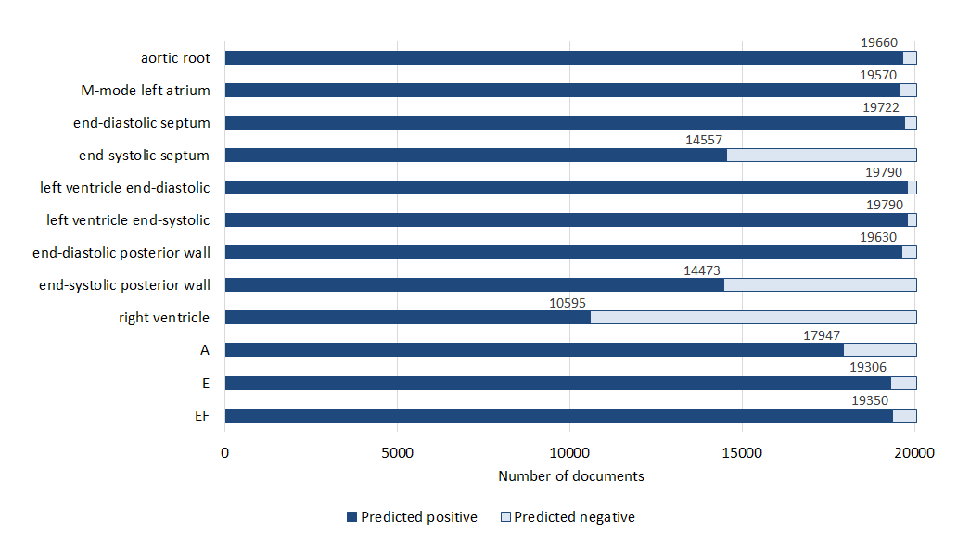
\includegraphics[width=\textwidth]{assets/figures/text_mining/extraction/ppv_npv.eps}
	\caption{Number of documents containing (predicted positive) and not containing (predicted negative) the given term. % The whole dataset contained 20,074 documents.
 }
	\label{fig:ppv_and_npv_values} 
\end{figure}

Figure \ref{fig:ppv_and_npv_values} shows that for eight echocardiography parameters, the algorithm could extract the measurement results from more than 19,000 reports. For these parameters, the relative frequencies were as follows: aortic root diameter: \SI{97.9}{\percent}, M-mode left atrial diameter: \SI{97.5}{\percent}, end-diastolic septum thickness: \SI{98.2}{\percent}, left ventricle end-diastolic diameter: \SI{98.6}{\percent}, left ventricle end-systolic diameter: \SI{98.6}{\percent}, end-diastolic posterior wall thickness: \SI{97.8}{\percent}, E-wave: \SI{96.2}{\percent}, and EF: \SI{96.4}{\percent}. Relevant information for the remaining four parameters could be extracted from fewer documents as these parameters are measured less frequently during echocardiography examinations. This was also confirmed by a medical expert. The relative frequencies for these are: end-systolic septum thickness: \SI{72.5}{\percent}; end-systolic posterior wall thickness: \SI{72.1}{\percent}; right ventricle end-diastolic diameter: \SI{52.8}{\percent}; A-wave: \SI{89.4}{\percent}.

In the next phase, the quality of the information extraction algorithm was evaluated. 100 reports having predicted positive labels and 100 reports with predicted negative labels have been randomly selected for each investigated term for evaluation purposes. Following this, these 2,400 selected reports have been manually evaluated, and they were labelled with true positive (TP), false positive (FP), true negative (TN) and false negative (FN) labels according to the comparison between the actual content of the document and the prediction. Using these results, numerous evaluation metrics, like sensitivity, specificity, positive predictive value (PPV, precision), negative predictive value (NPV), accuracy, balanced accuracy (Bal. acc.), and F1 score have also been calculated. The values of the calculated metrics can be seen in Table \ref{tab:extraction_evaluation_proposed}. All values are rounded to three decimal places.

\begin{table}[h!]
	\caption{Evaluation of the effectiveness of the proposed text mining-based information extraction method. % The table shows the number of positively predicted documents (\#PP) and the number of negatively predicted documents (\#PN) by terms. Furthermore, it contains the following quality measures regarding the results of the proposed information extraction method: sensitivity, specificity, positive predictive value (PPV), negative predictive value (NPV), accuracy, balanced accuracy (Bal. acc.), and F1 score.
	}
	\label{tab:extraction_evaluation_proposed}
	\centering
	\resizebox{\textwidth}{!}{
		\begin{tabular}{ lrrcccccccc}
			\toprule
			                             & \#PP  & \#PN & Sensitivity & Specificity & PPV   & NPV   & Accuracy & Bal. acc. & F1    \\
			\midrule
			aortic root                  & 19660 & 414  & 0.877       & 1.000       & 1.000 & 0.860 & 0.930    & 0.939     & 0.935 \\
			M-mode left atrium           & 19553 & 521  & 0.813       & 1.000       & 1.000 & 0.770 & 0.885    & 0.907     & 0.897 \\ 
			end-diastolic septum         & 19722 & 352  & 0.862       & 1.000       & 1.000 & 0.840 & 0.920    & 0.931     & 0.926 \\ 
			end-systolic septum          & 14557 & 5517 & 1.000       & 1.000       & 1.000 & 1.000 & 1.000    & 1.000     & 1.000 \\ 
			left ventricle end-diastolic & 19790 & 284  & 0.926       & 1.000       & 1.000 & 0.920 & 0.960    & 0.963     & 0.962 \\
			left ventricle end-systolic  & 19790 & 284  & 0.943       & 1.000       & 1.000 & 0.940 & 0.970    & 0.972     & 0.971 \\
			end-diastolic posterior wall & 19630 & 444  & 0.775       & 1.000       & 1.000 & 0.710 & 0.855    & 0.888     & 0.873 \\ 
			end-systolic posterior wall  & 14473 & 5601 & 1.000       & 1.000       & 1.000 & 1.000 & 1.000    & 1.000     & 1.000 \\ 
			right ventricle              & 10595 & 9479 & 0.980       & 1.000       & 1.000 & 0.980 & 0.990    & 0.990     & 0.990 \\ 
			A                            & 17947 & 2127 & 0.855       & 1.000       & 1.000 & 0.830 & 0.915    & 0.927     & 0.922 \\
			E                            & 19308 & 766  & 0.909       & 1.000       & 1.000 & 0.900 & 0.950    & 0.955     & 0.952 \\ 
			EF                           & 19525 & 549  & 0.901       & 1.000       & 1.000 & 0.890 & 0.945    & 0.951     & 0.948 \\ 
			\bottomrule
			Average                      &       &      & 0.904       & 1.000       & 1.000 & 0.887 & 0.939    & 0.952     & 0.948 \\
			\bottomrule
			%\bottomrule
		\end{tabular}
	}
\end{table}

In Table \ref{tab:extraction_evaluation_proposed}, we can see that both specificities and predicted positive values are equal to 1.0 for each parameter. It means that there were no false positive results predicted. The sensitivity of the proposed method takes values from 0.775 to 1.0, and the average sensitivity for the 12 measurements is 0.904. The accuracy of the algorithm varies between 0.855 and 1.0, and the average accuracy is 0.939. The balanced accuracy takes values between 0.888 and 1.0, and its average value is 0.952. The F1 score also shows sufficiently high values, it takes values between 0.873 and 1.0, and its average value is 0.948. The best results were obtained for end-systolic septum thickness and end-systolic posterior wall thickness. Results show that the most difficult parameter to obtain was the end-diastolic posterior wall thickness. At the same time, the extraction of the measurement result of ejection fraction as an essential diagnostic measure shows good results with 0.901 sensitivity, 1.00 specificity, 0.945 accuracy, and 0.948 F1 score values.

In the next phase of the evaluation, the false negative documents were examined in detail. The errors were classified into two types: (1) the parameter under study is included in the document and its measured value was recorded with numerical values ($Err_{num}$) or (2) the parameter under study is recorded in the document, but only textual information is given for it (e.g. "end-diastolic posterior wall: can not be measured") ($Err_{text}$). Table \ref{tab:number_of_errors} shows the occurrence of two different types of error by terms. Findings that contain only textual information on the parameter under study mainly were found for the A-wave. In the case of this type of error ($Err_{text}$), the algorithm could not be expected to extract the correct information from the document since the proposed method only aims to extract numerical measurement results. However, in a higher proportion of false negative cases, reports also contained numeric measurement results. This is most noticeable for terms end-diastolic posterior wall thickness with 27 occurrences and left atrium diameter with 22 occurrences. Therefore, this error type has been further analysed.

\begin{table}[h]
	\caption{Frequency of different error types in false negative documents. %While in some cases, the reason for the error was that reports contained only text information about the echocardiography parameter ($Err_{text}$), in most cases, reports also contained numeric values ($Err_{num}$).
	}
	\label{tab:number_of_errors}
	\centering
	\begin{tabular}{ lrr }
		\toprule
		                             & $Err_{num}$ & $Err_{text}$ \\
		\midrule
		aortic root                  & 5           & 9            \\
		M-mode left atrium           & 22          & 1            \\
		end-diastolic septum         & 12          & 3            \\
		end-systolic septum          & 0           & 0            \\
		left ventricle end-diastolic & 6           & 2            \\
		left ventricle end-systolic  & 6           & 0            \\
		end-diastolic posterior wall & 27          & 0            \\
		end-systolic posterior wall  & 0           & 0            \\
		right ventricle              & 1           & 1            \\
		A                            & 0           & 17           \\
		E                            & 10          & 0            \\
		EF                           & 10          & 1            \\
		\midrule
		Total                        & 99          & 34           \\
		\bottomrule
	\end{tabular}
\end{table}

Table \ref{tab:error_details} shows the detailed presentation of the classification of $Err_{num}$ errors according to their causes. The causes of the errors were classified into the following six categories.

\begin{itemize}
	\item \textit{missing whitespaces}: there were missing whitespaces in the recorded text (e.g. "aortic root: 26mmleft atrium: 47 mm"); 
	\item \textit{multiple values}: there were several measurement results recorded together, therefore the term could not be successfully extracted (e.g. "aorta anulus-sinus valsalva-root: 26-36-33 mm"); 
	\item \textit{additional text}: the recorded information contained additional text (e.g. "Aortic root: calcified, 26 mm");
	\item \textit{defined by other parameters}: the measurement result was given in the document as it is equal to another measurement result (e.g. "E=A"); 
	\item \textit{wrong order}: the order of the measurement value and its unit was wrong (e.g. "mm7");
	\item \textit{wrong format}: the recording format of the measured value does not meet the preliminary expectations (e.g. "left atrium: x47 mm", "left atrium 55xmm", "left atrium: 34x33x40 mm"). 
\end{itemize}

\begin{table}[h]
	\caption{Causes of the error type $Err_{num}$ in false negative documents.
		%In most cases, the error arose from missing whitespace characters, recording additional text information, and recording multiple measurement results together.
	}
	\label{tab:error_details}
	\centering
	\resizebox{\textwidth}{!}{
		\begin{tabular}{lcccccc|r }
			\toprule
			                             & missing     & multiple & additional & defined by      & wrong & wrong  & \multirow{2}{*}{total} \\
			                             & whitespaces & values   & text       & other parameter & order & format &                        \\
			\midrule
			aortic root                  & 0           & 0        & 5          & 0               & 0     & 0      & 5                      \\
			M-mode left atrium           & 0           & 7        & 11         & 0               & 0     & 4      & 22                     \\
			end-diastolic septum         & 10          & 2        & 0          & 0               & 0     & 0      & 12                     \\
			left ventricle end-diastolic & 5           & 0        & 1          & 0               & 0     & 0      & 6                      \\
			left ventricle end-systolic  & 6           & 0        & 0          & 0               & 0     & 0      & 6                      \\
			end-diastolic posterior wall & 22          & 2        & 0          & 0               & 3     & 0      & 27                     \\
			right ventricle              & 0           & 0        & 1          & 0               & 0     & 0      & 1                      \\
			E                            & 0           & 0        & 2          & 8               & 0     & 0      & 10                     \\
			EF                           & 0           & 0        & 10         & 0               & 0     & 0      & 10                     \\
			\bottomrule
			total                        & 43          & 11       & 30         & 8               & 3     & 4      &                        \\
						 
		\end{tabular}
				
	}
\end{table}

As it can be seen in Table \ref{tab:error_details}, the top three most frequent reasons for classification error were lack of whitespace characters in the text (43 occurrences), measurement values recorded with additional text (30 occurrences), and multiple measurement results recorded together (11 occurrences). However, it is also clear that not only general errors were found but also errors specific to the parameters. For example, the difficulty in extracting the M-mode left atrial diameter is mainly because the used measurement method is not well defined, and in some cases, 2D measurement was applied. Another typical example is the recording of the value of ejection fraction, which is often only given as an estimated value (e.g. "EF: estimated \SI{68}{\percent}"). Knowledge of this and similar facts could greatly facilitate the development of a postprocessing method that could further reduce the number of false negative documents. 

\subsection{Discussion of the results}
\label{sec:patterson_comparison}

The main advantage of the suggested method is that it extracts the measurement results of cardiac ultrasound findings by automatically identifying the text fragments describing the measurement names. For this purpose, it uses an expert-defined dictionary and applies text-similarity mappings to identify the unified name of the measurement. In contrast, methods published in the literature typically perform regex-based information extraction, which searches for information based on a priori assumptions. In these methods, the set of regular expressions has to be defined for each measurement parameter separately, which requires IT skills. Furthermore, regular expressions are created as a result of lengthy iterative manual modifications.

To show the effectiveness of the proposed method in terms of finding the measurement descriptions, a comparative analysis between the direct search and the suggested method was performed. All the dictionary elements used in my study were searched in the document set during this analysis, and the evaluation was performed manually on the same test set. As a part of the comparative analysis, I manually checked whether any related numerical measurement results were recorded in the documents. The direct search results are presented in Table \ref{tab:extraction_evaluation_proposed_direct}. All values are rounded to three decimal places.

\begin{table}[h!]
	\caption{Evaluation of the effectiveness of direct search. %The table shows the number of positively predicted documents (\#PP) and the number of negatively predicted documents (\#PN) by terms. Furthermore, it contains the following quality measures regarding the results of the proposed information extraction method: sensitivity, specificity, positive predictive value (PPV), negative predictive value (NPV), accuracy, balanced accuracy (Bal. acc.), and F1 score. All results are rounded to three decimal places.
	}
	\label{tab:extraction_evaluation_proposed_direct}
	\centering
	\resizebox{\textwidth}{!}{
		\begin{tabular}{ lrrcccccccc}
			\toprule
			                             & \#PP  & \#PN  & Sensitivity & Specificity & PPV   & NPV   & Accuracy & Bal. acc. & F1    \\
			\midrule
			aortic root                  & 19708 & 366   & 0.902       & 0.843       & 0.830 & 0.910 & 0.870    & 0.872     & 0.865 \\
			M-mode left atrium           & 19853 & 221   & 0.941       & 0.826       & 0.800 & 0.950 & 0.875    & 0.884     & 0.865 \\ 
			end-diastolic septum         & 14870 & 5204  & 0.521       & 1.000       & 1.000 & 0.080 & 0.540    & 0.760     & 0.685 \\ 
			end-systolic septum          & 25    & 20049 & 0.217       & 1.000       & 1.000 & 0.100 & 0.280    & 0.609     & 0.357 \\
			left ventricle end-diastolic & 3939  & 16135 & 0.511       & 0.700       & 0.970 & 0.070 & 0.520    & 0.605     & 0.669 \\
			left ventricle end-systolic  & 4096  & 15978 & 0.146       & 0.124       & 0.150 & 0.120 & 0.135    & 0.135     & 0.148 \\
			end-diastolic posterior wall & 14858 & 5216  & 0.556       & 0.681       & 0.850 & 0.320 & 0.585    & 0.618     & 0.672 \\ 
			end-systolic posterior wall  & 2     & 20072 & 0.020       & 0.600       & 0.500 & 0.030 & 0.048    & 0.310     & 0.038 \\ 
			right ventricle              & 12070 & 8004  & 0.941       & 0.950       & 0.950 & 0.940 & 0.945    & 0.945     & 0.945 \\ 
			A                            & 19978 & 96    & 0.023       & 0.093       & 0.020 & 0.104 & 0.061    & 0.058     & 0.021 \\
			E                            & 19903 & 171   & 1.000       & 0.806       & 0.760 & 1.000 & 0.880    & 0.903     & 0.864 \\ 
			EF                           & 19764 & 310   & 0.918       & 0.809       & 0.780 & 0.930 & 0.855    & 0.863     & 0.843 \\ 
			\bottomrule
			Average                      &       &       & 0.558       & 0.703       & 0.718 & 0.463 & 0.550    & 0.630     & 0.581 \\
			\bottomrule
		\end{tabular}
	}
\end{table}

Comparing the results of Table \ref{tab:extraction_evaluation_proposed} and Table \ref{tab:extraction_evaluation_proposed_direct}, we can see that the proposed method performed better in extracting all measurement descriptions. This is, of course, due to the fact that the proposed methodology also includes a text similarity mapping, which can improve the results significantly. In the case of the "end-systolic septum" and "end-systolic posterior wall", the direct search has found only a few search results. In these cases, the text similarity mapping and the EPC refinement phases yielded excellent results in the proposed methodology. In the case of the A-wave, the main problem was, of course, caused by the fact that "A" as a search term is part of the dictionary used, at the same time, it is also a definite article in Hungarian. The search for the terms "E" and "EF" also causes similar problems due to the brevity of the measurement terms. However, as these descriptions are indeed included as measurement descriptions in several documents, the discrepancy is less significant. Moreover, we have to note that the aim of the direct search was only to find the elements of the dictionary in the echocardiography documents, but the related measurement results were extracted manually. In contrast, the proposed method can find the measurement descriptions and extract the related measurement results. By manual refinement, the regex search could be refined, but as mentioned before, this requires the overview of a huge part of the documents, which is a time-consuming task and results in only corpus-dependent regex terms. 

\vspace{0.5cm}

If we consider the possibility of international comparison, we find that previously published methods often aim to extract the results of only a single measurement parameter. Hence, the complete comparative evaluation of the effectiveness of the proposed methodology is not feasible. While partial comparisons can be made regarding the extraction of a single ultrasound parameter, the evaluation of the results should consider that the aim of each method was typically different. For example, many previous studies aimed to extract the ejection fraction mentions, including numerical and text descriptions. In contrast, my method was designed to extract several parameters; but at the same time, it aimed at only the extraction of the numerical measurement result. 

Research presented in \cite{garvin2012automated} aimed at extracting EF values and mentions from echocardiography reports. The analysis was based on a regex search, and to measure the quality of the method, 765 reports were evaluated. For defining regex terms, a set of sample documents were visually analysed to determine the structure of the documents. The initial pattern set of the regex expressions defined directly for extracting EF values from the reports achieved only an F1=0.4387 score, but after several refinement phases of the regex expressions, the highest value was F1=0.9571. Finally, the sensitivity of the proposed whole system was 0.889, and the positive predicted value was 0.950. In contrast, my method achieved a sensitivity of 0.901, a positive predicted value of 1.0 and F1=0.948 when extracting EF values. Although the results can not be compared directly due to the issues mentioned before (my method was developed to not directly extract the EF values but simultaneously more echocardiography parameters), it can be seen that my method has achieved good results and is competitive.

In \cite{xie2017extracting}, a large number of echocardiography reports (621,856) were analysed, and the aim was to extract both the numerically or text-recorded ejection fraction measurement results. First, the text descriptions were searched based on a set of concepts defined by the experts, and then, the numerical values associated with the keyword were searched first backwards, then forwards, starting from the text description. If a numeric value was not found, predefined text descriptions (e.g. "severe") were also searched and extracted. The quality of the proposed method was evaluated based on 200 randomly selected reports manually. The algorithm (including the textual information extraction as well) got sensitivity=0.950 and PPV=0.969. Nevertheless, it should be noted that in the present case, we are talking about a system based on the definition and application of a large set of regex terms using a priori knowledge, and it was developed exclusively for the extraction of the ejection fraction and therefore only applicable to it. 

In the study presented in \cite{patterson2017unlocking}, the authors aimed to extract not only ejection fraction measurements but also other cardiac function measurements. The developed methodology was based on natural language processing using a dictionary lookup, rules, and patterns. In this study, the developed NLP method was again based on a large set of regex expressions fine-tuned for both the term and value identifications. The proposed method was evaluated not only for echocardiography reports but also for general clinical notes and radiology reports. Their evaluation was based on 100-100 documents of each type of record. The method achieved averaged F1 scores of 0.844 and averaged precision of 0.982 regarding the echocardiography datasets, respectively, for the investigated 27 measurements. For my method the average F1 score was 0.948 and the average precision was 1.000. A comparison of the extraction efficiency of the cardiac ultrasound parameters involved in both cases is shown in Table \ref{tab:comparison_patterson}. Table \ref{tab:comparison_patterson} contains only those results which are covered by both studies.

It can be seen that for some parameters, the method published in \cite{patterson2017unlocking} performed better, while for other parameters, the my proposed method gave better results. For the most informative cardiac ultrasound parameter (EF), the sensitivity of my proposed method was exactly 0.1 better than the method proposed in \cite{patterson2017unlocking}, and the PPV values were identical (1.0) for both methods.

\begin{table}[h!]
	\caption{Comparison of results of my text mining-based information extraction method with the results achieved by the method presented by Patterson.}
	\label{tab:comparison_patterson}
	\centering
	\resizebox{\textwidth}{!}{
		\begin{tabular}{lcccc}
			\toprule
			& \multicolumn{2}{c}{Results from Patterson} & \multicolumn{2}{c}{My results} \\
			                             & sensitivity & PPV   & sensitivity & PPV   \\
			\midrule
			end-diastolic septum         & 1.000       & 0.926 & 0.862       & 1.000 \\
			left ventricle end-diastolic & 0.706       & 1.000 & 0.926       & 1.000 \\
			left ventricle end-systolic  & 1.000       & 1.000 & 0.943       & 1.000 \\
			end-diastolic posterior wall & 0.842       & 0.970 & 0.775       & 1.000 \\
			EF                           & 0.801       & 1.000 & 0.901       & 1.000 \\
			\bottomrule
		\end{tabular}
	}
\end{table}

Evaluating the results, we can see that the proposed method provides similar or better results than other methods published in the literature. However, the methods published in the literature typically rely on the use of regex-based expressions, of which the preparation requires prior knowledge of the contents of the documents. In contrast, my method is simple, does not require the definition of regex expressions and does not rely on any assumptions about the form in which the results are recorded. Moreover, though my proposed method can extract many numeric measurement results, it still achieves similar results when compared to the methods that are designed to extract only one specific measurement result.

Like with other methods, my method also has some limitations. First, with the proposed method, only numerical measurement results can be extracted; textual descriptions regarding the measurements cannot. If numerically recorded measurement results are supplemented with textual descriptions (e.g. "Aortic root: calcified, 26 mm"), this additional information remains hidden. Additional text information, unusual recording formats and missing spaces can also cause errors when extracting measurement results from the text. However, it should be noted that these errors do not always cause problems. Furthermore, measurement results recorded by another echocardiography result (e.g. "E=A") will be missing from the extracted results. However, the mentioned limitations can be generally eliminated by extending the proposed general methodology with special rules. 

\section{Related theses}

\subsection*{Thesis 2.1}

I examined and compared different text similarity metrics applied in the field of NLP to determine which similarity metrics present the highest gain in terms of extracting medical terms from echocardiography documents. The examined metrics were the following: Longest Common Subsequence, Levenshtein distance, weighted Levenshtein distance, Jaro-Winkler distance and cosine distance. I established that the Jaro-Winkler distance is the most suitable to identify medical terms in echocardiography documents.

\subsection*{Thesis 2.2}

By utilising the findings of the comparison of different text similarity metrics, I proposed a text mining-based information extraction method to extract numerical measurement results from echocardiography documents. The proposed method performs generally applicable, language-independent text-cleaning preprocessing activities, automatically identifies measurement names and results, and returns them in a structured way. The methodology is also able to identify, correct and unify synonyms, acronyms, and typos. Since the method does not contain any language-dependent implementation elements, it is suitable for processing echocardiography findings written in any language.

\subsection*{Thesis 2.3}

The proposed text mining-based information extraction method was evaluated on a document set containing more than 20,000 echocardiography reports. During the evaluation, 12 relevant echocardiography parameters were extracted from the documents. As a result, an average sensitivity of 0.904, an average specificity of 1.0 and an average F1 score of 0.948 were obtained. The evaluation sufficiently demonstrated the broad applicability of the method, also confirmed by the experts.

\subsection*{Related publications}

\begin{itemize}
	\item[\textbf{P10}] Szabolcs Szekér and Ágnes Vathy-Fogarassy. Application of Text Mining Methods on Unstructured Hungarian Echocardiogram Documents. \textit{Proceedings of the Pannonian Conference on Advances in Information Technology (PCIT 2019)}, University of Pannonia, pages 187-193, 2019. 
	\item[\textbf{P11}] Szabolcs Szekér, György Fogarassy, Károly Machalik, and Ágnes Vathy-Fogarassy. Application of named entity recognition methods to extract information from echocardiography reports. \textit{Studies in Health Technology and Informatics}, Vol. 260, pages 41–48, 2019. (Q3)
	\item[\textbf{P12}] Ágnes Vathy-Fogarassy, Szabolcs Szekér, Balázs Szolár, and György Fogarassy. The efficiency of different distance metrics for keyword-based search in medical documents: A short case study. \textit{Studies in Health Technology and Informatics}, Vol. 271, pages 232–239, 2020. (Q3) 	      	
	\item[\textbf{P13}] Szabolcs Szekér, György Fogarassy, and Ágnes Vathy-Fogarassy. A general text mining method to extract echocardiography measurement results from echocardiography documents. \textit{Artificial Intelligence in Medicine}, 143: 102584, 2023. (D1, IF: 7.5)
\end{itemize}
